%*******************************************************************************
%****************************** Second Chapter *********************************
%*******************************************************************************

\chapter{Cell segmentation}

\ifpdf
    \graphicspath{{Chapter2/Figs/Raster/}{Chapter2/Figs/PDF/}{Chapter2/Figs/}}
\else
    \graphicspath{{Chapter2/Figs/Vector/}{Chapter2/Figs/}}
\fi

%********************************** %First Section  **************************************
\section{Basics of image manipulation}

\subsection{Image manipulation overview}

\begin{figure}[htbp!]
\centering
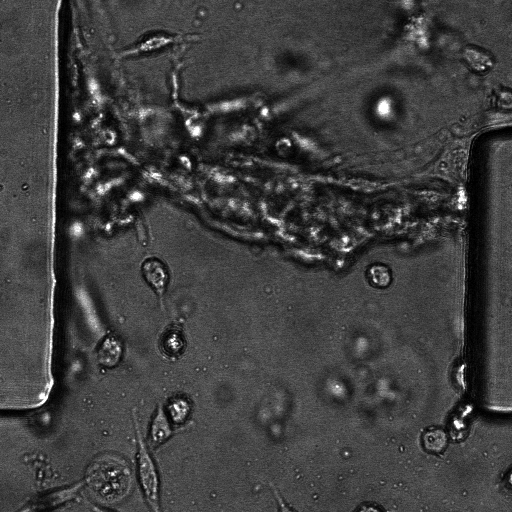
\includegraphics[width=1.0\textwidth]{211-digital_image_sample_bf-050714_s13_ch1_t85_z30}
\caption[Brightfield image sample]{An example of a typical Brightfield image taken with a confocal microscope.}
\label{fig:digital_image_sample_bf}
\end{figure}

The ability to segment cells is dependent on a mathematical description of digital images. Images are stored as 2D arrays of pixel intensities [ref]. Specifying two coordinates will access a single intensity value. This can be thought of as a matrix and is subject to many of the same algebra and element-wise operations. Image manipulation is the use of various algorithmic techniques to mathematically describe features and search for similar patterns within image data.

We use the term "pixel" in this paper to refer specifically to the data structure that holds one of these intensity values, not to the physical surface section in a detector. The data structure can be visualised as a parking space, into which "cars" (intensity values) are inserted. In this analogy, an image data structure is a large rectangular car park. An example of a Brightfield image is shown in Figure~\ref{fig:digital_image_sample_bf}.

In this section, several key techniques are described that allow images to be segmented. Edge detection allows the boundaries between an object and the background to be identified. A blob is a continuous region of similar colour that can be contained inside an object or form part of the background. More complex features such as corners can be identified by increasingly specific search algorithms. Images and other data can be subjected to repeated machine learning techniques to identify objects more consistently.

\subsection{Edge detection}

\begin{figure}[htbp!]
\centering
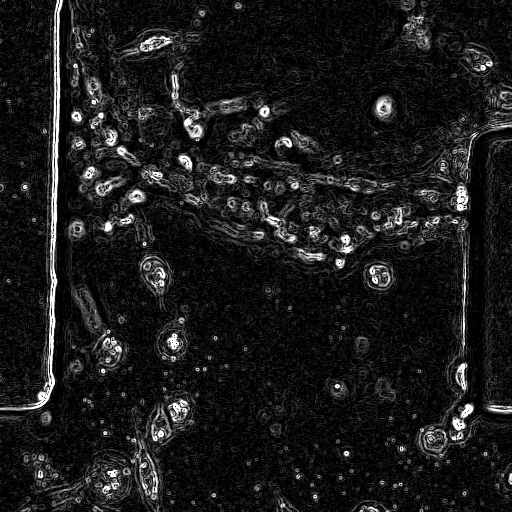
\includegraphics[width=1.0\textwidth]{212-canny_bf-050714_s13_ch1_t85_z30}
\caption[The canny filter]{Edges can be found using the Canny Edge Detection Filter.}
\label{fig:canny_filter_bf}
\end{figure}

An edge in a 2d image can be described as an "intensity discontinuity" [ref] between two regions. This discontinuity can be described mathematically, and can be approximated by a number of functions, such as the commonly-used Laplacian of Gaussian function [ref]. Through convolution, parts of the image that share the same functional form as the approximating function can be highlighted and deemed to be edge pixels. A popular formalisation of this method is known as the Canny edge detection filter. This works by combining information about the directionality as well as the intensity of edges [ref]. An example of this method applied to a Brightfield image is shown in Figure~\ref{fig:canny_filter_bf}.

\subsection{Blobs}

\begin{figure}[htbp!]
\centering
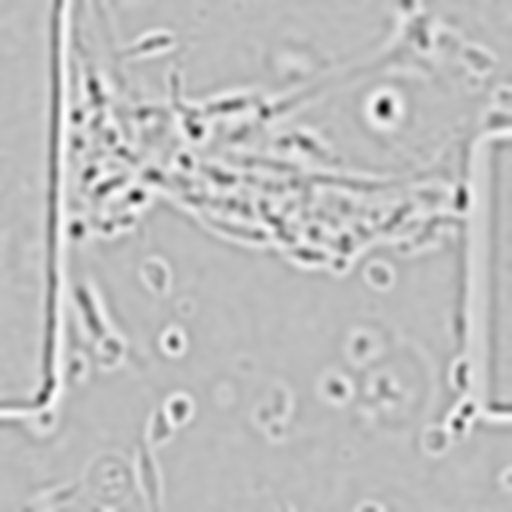
\includegraphics[width=1.0\textwidth]{213-blobs_bf-050714_s13_ch1_t85_z30}
\caption[Blob detection]{Contiguous blobs of colour can be found using a Gaussian filter.}
\label{fig:blob_detection_bf}
\end{figure}

A blob is a continuous region of uniform colour in an image. "Uniform" means a single colour or slight variations around a single colour. Blobs are often associated with objects. A blob could represent the interior of a cell object, for example. Different objects that share similar properties might contain blobs of similar size or shape. In a similar way to edges, blobs can be convolved with an approximating function, often a Gaussian kernel [ref]. A Gaussian kernel of a defined size will highlight blobs of a similar size, as shown in Figure~\ref{fig:blob_detection_bf} using a Gaussian filter of size 5 pixels. Boundaries between blobs are edges.

\subsection{Complex features and machine learning}

Blobs and edges can be combined into a generalised model of a an object, such as a cell [ref]. When two edges meet at a point, this can be recognised as a corner. Machine learning uses repeated training techniques to allow information stored about previously observed cells to improve recognition of cells present in new data. They can combine information about cell features, like blobs and edges, into much more complex models of a cell.

%********************************** %Second Section  **************************************
\section{Basics of cell segmentation}

\subsection{Optical structure of the cell}

A typical animal cell is both colourless and transparent [ref]. It is made up of a sheath of protein containing the cytoplasm of a cell and other cell structures like the nucleus and the cell skeleton. When observed using white light, the light will pass through most of the cell, but some light will be blocked when viewing parts of the cell tangential to its surface, leading to the appearance of an edge.

\subsection{Cell shape}

Cell shape is highly variable and unpredictable, but it is generally composed of a circular region surrounding the nucleus. It also has various extensions of the cell wall, dubbed "protrusions", that allow the cell to move [ref]. These protrusions provide the greatest amount of information about the behaviour of the cell and are the focus of this project in terms of segmentation. This requires that the protrusions be associated with the correct cell.

\subsection{Fluorescence microscopy}

To enhance contrast, cells are often stained with a fluorescent substance that can be excited by a laser and make the cells more visible. Most staining methods require the cells to be fixed, but a few, including Green Fluorescent Protein (GFP), can be used during live cell imaging [ref]. GFP highlights the cytoplasm of the cell [ref]. There are other staining substances that can highlight different parts of the cell such as the nucleus or the cytoskeleton. It should be noted that the distribution of intensity values within cell interiors or cell edges may be very different from cell to cell and from frame to frame.

\subsection{Cell segmentation errors}

Cell segmentation algorithms use a variety of image processing techniques. A common approach is to start at a particular pixel (often chosen by a human user) and examine intensity values in neighbouring pixels. The algorithm will then decide whether or not an adjacent pixel belongs to the same object as the original pixel. Various parameter settings govern this choice. Often, this algorithm is recursive. If an adjacent pixel is added to the cell data object, the algorithm will restart at that adjacent pixel. This can lead the cell object spilling over unclear cell edges, since the algorithm does not find a clear place to stop. This is shown in Figure~\ref{fig:cell_segmentation_errors} This is a common problem in cell segmentation and often occurs in cell protrusions, where the intensity values may shade smoothly into the background noise.

\begin{figure}[htbp!]
\centering
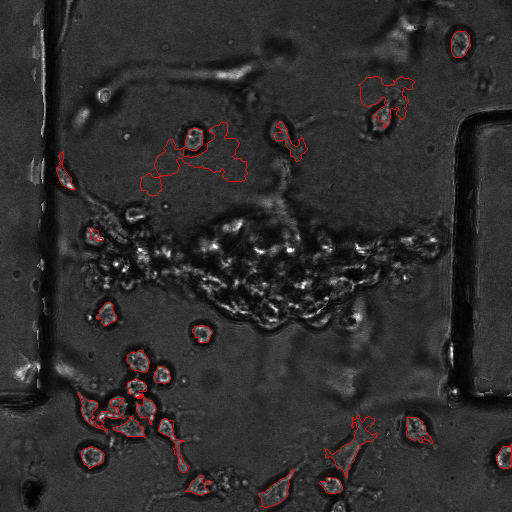
\includegraphics[width=1.0\textwidth]{bad_segmentation-tile_050714_s13_ch-zbf-8-5-5-outline-zcomp-8-1-1-zedge-8-1-1-YUZ29SWD_t2}
\caption[Cell segmentation error examples]{Examples of cell segmentation errors. Cell recognition extends into the background if the edge is not clearly defined.}
\label{fig:cell_segmentation_errors}
\end{figure}

In the group of three cells at the top of the image, all three of the recognitions fail, as the segmentation spills out of the cells into the background. We refer to these as segmentation errors or mis-recognitions.

%********************************** %Third Section  **************************************
\section{Review of studies on cell segmentation}

\subsection{Studies using GFP fluorescence data}

Cell segmentation studies using GFP fluorescence data focus on easily identifiable cell features such as the nucleus. Various problems are noted in these studies. The first is the GFP glare, where other materials in the environment reflect fluorescence. Other materials can sometimes generate fluorescence themselves. High noise levels are often encountered.

The GFP images are often not very sharp. Some studies have attempted to sharpen the images by passing them through a high-pass spatial filter. Unfortunately, this also amplifies the noise. One study [ref: Arce] experimented with using a low-pass spatial filter to sharpen the image and simultaneously reducing the noise via a mathematical technique. Arce et al. note that thresholding can also be used to reduce noise, but also that ``it can omit low-intensity parts of cells".

Another study [ref: Rizk] used an approximation of the point spread function (or PSF) of the microscope hardware to deconvolve the images and correct for lens aberrations that might also cause noise-like effects and/or lower quality images.

\subsection{Studies using brightfield data}

Most studies that attempt to use the Brightfield for segmentation note that in-focus images of objects in the Brightfield do not have sufficient contrast with the background to distinguish edges. One study [ref: Ali] attempted to use a focus level that was slightly out of focus to locate the edges and separate different cells. They try to find the focus using the entropy of the whole image. They also consider several different types of textures (spatial frequencies) inside the cells.

\subsection{Studies using confocal imaging}

The study by Selinummi et all [ref] attempts to use the Brightfield 3D profile to increase the contrast in the Brightfield image data. They assume that the presence of a cell in an otherwise uniform background will cause a disturbance in the shape of the 3D profile. Thus, the standard deviation of this disturbance can be used to indicate the presence of a cell.

Two studies [ref: Zanella, Liu] segment 3D images using a spherical Hough transform, which highlights centres of spheres with a particular radius, marking potential cell candidates.

\subsection{Review of studies}

Current state-of-the-art segmentation requires human interaction and long processing time due to high resolution. The studies here tend to sacrifice human interaction and resolution for high throughput. They employ various techniques to raise the accuracy of the segmentation given these two constraints to allow accurate cell boundaries to still be identified.

The methods reviewed here of preprocessing image data and performing cell segmentation have several limitations. The first is the significant effect of image noise on segmentation accuracy and the unreliability of most image de-noising techniques. Another problem is the lack of contrast when using Brightfield images that prevent edges from being recognised. Finally, a related issue is the ineffectiveness of thresholding with regard to differentiating between a cell and the background, since different parts of the cell might have different pixel intensity values.
